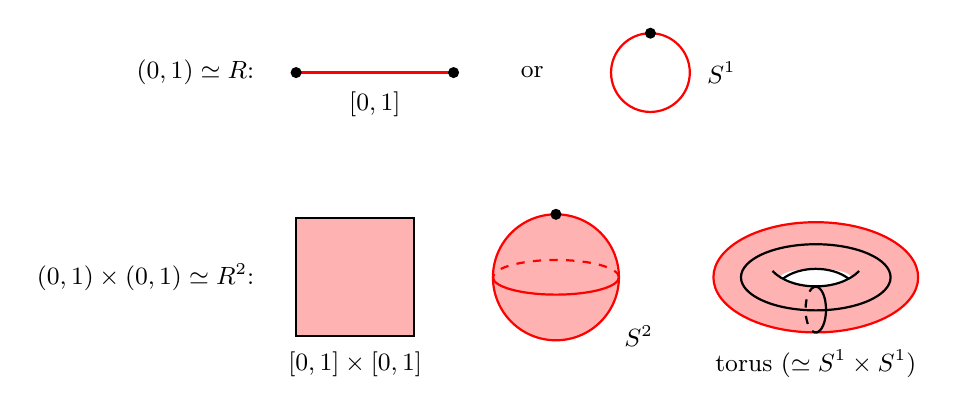
\begin{tikzpicture}[line width=0.8pt, every node/.style={font=\small}]
  % (0,1) ~ R compactifies to [0,1] or S^1
  \node[anchor=east] at (-0.4,2.6) {$(0,1)\simeq\mathbb{R}$:};
  \draw[red, line width=1.2pt] (0,2.6) -- (2,2.6);
  \fill (0,2.6) circle (2pt) (2,2.6) circle (2pt);
  \node at (1,2.2) {$[0,1]$};
  \node at (3,2.6) {or};
  \draw[red] (4.5,2.6) circle (0.5);
  \fill (4.5,3.1) circle (2pt);
  \node at (5.4,2.6) {$S^1$};
  % (0,1)x(0,1) ~ R^2
  \node[anchor=east] at (-0.4,0) {$(0,1)\times(0,1)\simeq\mathbb{R}^2$:};
  \fill[red, fill opacity=0.3] (0,-0.75) rectangle (1.5,0.75);
  \draw (0,-0.75) rectangle (1.5,0.75);
  \node at (0.75,-1.1) {$[0,1]\times[0,1]$};
  % sphere
  \fill[red, fill opacity=0.3] (3.3,0) circle (0.8);
  \draw[red] (3.3,0) circle (0.8);
  \draw[red] (2.5,0) arc[start angle=180, end angle=360, x radius=0.8, y radius=0.22];
  \draw[red, dashed] (4.1,0) arc[start angle=0, end angle=180, x radius=0.8, y radius=0.22];
  \fill (3.3,0.8) circle (2pt);
  \node at (4.35,-0.75) {$S^2$};
  % torus
  \fill[red, fill opacity=0.3, even odd rule] (6.6,0) ellipse (1.3 and 0.7) (6.6,0.0) ellipse (0.45 and 0.11);
  \draw[red] (6.6,0) ellipse (1.3 and 0.7);
  \draw (6.05,0.08) .. controls (6.3,-0.18) and (6.9,-0.18) .. (7.15,0.08);
  \draw (6.18,-0.02) .. controls (6.4,0.15) and (6.8,0.15) .. (7.02,-0.02);
  \draw (6.6,0) ellipse (0.95 and 0.42);
  \draw (6.6,-0.7) arc[start angle=-90, end angle=90, x radius=0.13, y radius=0.29];
  \draw[dashed] (6.6,-0.12) arc[start angle=90, end angle=270, x radius=0.13, y radius=0.29];
  \node at (6.6,-1.1) {torus ($\simeq S^1\times S^1$)};
\end{tikzpicture}
